\documentclass[12pt,a4paper]{article}
\usepackage{geometry}
\geometry{left=2.5cm,right=2.5cm,top=2.0cm,bottom=2.5cm}
\usepackage[english]{babel}
\usepackage{amsmath,amsthm}
\usepackage{amsfonts}
\usepackage[longend,ruled,linesnumbered]{algorithm2e}
\usepackage{fancyhdr}
\usepackage{ctex}
\usepackage{array}
\usepackage{longtable}
\usepackage{listings}
\usepackage{color}
\usepackage{graphicx}
\graphicspath{{figures/}}
\lstset{
  basicstyle=\ttfamily\small,
  breaklines=true,
  columns=fullflexible,
  frame=single,
  keepspaces=true,
  numbers=left,
  numbersep=6pt,
  numberstyle=\tiny,
  showstringspaces=false
}

\begin{document}


\title{
{《优化理论与算法》第12次作业
}
}
\date{}

\author{
 姓名：\underline{焦传斌}~~~~~~
学号：\underline{2024111223}~~~~~~}

\maketitle
\begin{itemize}
	\item 作业截止于{\bf 周五（6/5/2026）}，在Canvas系统中提交PDF或照片文件
	\item 作业题目的tex文件可以在Canvas中下载
	\item 鼓励相互讨论，但不要抄袭.
\end{itemize}
%%%%%%%%%%%%%%%%%%%%%%%%%%%%%%%%%%%%%%%%%%%%%%%%%%%%%%%%%%%%%%%%%
%%%%%%%%%%%%%%%%%%%%%%%%%%%%%%%%%%%%%%%%%%%%%%%%%%%%%%%%%%%%%%%%%



\section{一阶算法}

\paragraph{1.1}  给定$\lambda>0, x\in \mathbb{R}^n$，考虑如下函数形式（岭回归问题）
$$\min f(x)=\frac{1}{2} \|Ax-b\|^2_2+\lambda \|x\|_2^2$$
\begin{itemize}
	\item 最优解$x^*$的显示表达式是什么?
	\item 如果利用梯度下降法，其迭代算法框架是什么？
	\item 如果利用随机梯度下降法，其迭代算法框架是什么？
	\item 对比上述三种方法的优劣。
\end{itemize}

\textbf{解：}
设 $A\in\mathbb R^{m\times n}$，第 $i$ 行记为 $a_i^T$。目标函数为
\[
  f(x)=\frac12\|Ax-b\|_2^2+\lambda\|x\|_2^2 .
\]
其梯度和 Hessian 分别为
\[
  \nabla f(x)=A^T(Ax-b)+2\lambda x,
  \qquad
  \nabla^2 f(x)=A^TA+2\lambda I.
\]
由于 $\lambda>0$，有 $A^TA+2\lambda I\succ0$，所以该问题是强凸二次优化问题，最优解唯一。由一阶最优性条件
\[
  A^T(Ax^\star-b)+2\lambda x^\star=0
\]
得到
\[
  (A^TA+2\lambda I)x^\star=A^Tb,
  \qquad
  \boxed{
  x^\star=(A^TA+2\lambda I)^{-1}A^Tb } .
\]

如果使用梯度下降法，先选取初始点 $x^0$、步长序列 $t_k>0$ 和停止精度 $\varepsilon$，然后迭代
\[
  g^k=\nabla f(x^k)=A^T(Ax^k-b)+2\lambda x^k,
\]
\[
  x^{k+1}=x^k-t_kg^k.
\]
因为本题 Hessian 为常矩阵，梯度 Lipschitz 常数可以取
\[
  L=\lambda_{\max}(A^TA)+2\lambda.
\]
固定步长可取 $0<t<2/L$，常用 $t=1/L$。对二次函数也可以使用精确线搜索：
\[
  t_k=\frac{(g^k)^Tg^k}{(g^k)^T(A^TA+2\lambda I)g^k}.
\]
当 $\|g^k\|_2\leq\varepsilon$ 或迭代次数达到上限时停止。

如果使用随机梯度下降法，把残差项按样本行拆开。每次随机抽取指标 $i_k\in\{1,\ldots,m\}$，则一个无偏随机梯度可以取为
\[
  \tilde g^k
  =
  m(a_{i_k}^Tx^k-b_{i_k})a_{i_k}+2\lambda x^k,
  \qquad
  \mathbb E[\tilde g^k\mid x^k]=\nabla f(x^k).
\]
于是 SGD 迭代为
\[
  x^{k+1}=x^k-\eta_k\tilde g^k.
\]
 mini-batch $B_k$：
\[
  \tilde g^k
  =
  \frac{m}{|B_k|}
  \sum_{i\in B_k}(a_i^Tx^k-b_i)a_i
  +2\lambda x^k.
\]
SGD 的步长 $\eta_k$ 通常选为递减步长，例如 $\eta_k=\eta_0/\sqrt{k+1}$，或者在机器学习问题中选用小的常数步长并配合调参。

\begin{center}
\renewcommand{\arraystretch}{1.35}
\begin{tabular}{|p{2.3cm}|p{3.7cm}|p{3.7cm}|p{3.6cm}|}
\hline
方法 & 优点 & 缺点 & 适用场景 \\
\hline
显式解
& 一次求出精确最优解；不需要调步长；数值精度高
& 需要形成并求解 $(A^TA+2\lambda I)x=A^Tb$；当 $n$ 很大时矩阵存储和分解成本高
& 中小规模岭回归；需要高精度解的问题 \\
\hline
梯度下降
& 每步只需计算全梯度；实现简单；对强凸光滑问题线性收敛
& 每步要扫描全部样本；对条件数 $\kappa=L/\mu$ 敏感，病态问题中可能很慢
& 中等规模数据；矩阵求逆代价较高但全梯度可承受的问题 \\
\hline
随机梯度下降
& 单步计算便宜；适合大样本和在线数据；内存需求低
& 梯度有噪声，函数值会震荡；通常只能以递减步长渐近收敛；对学习率较敏感
& 大规模机器学习、在线学习、样本不断到达的场景 \\
\hline
\end{tabular}
\end{center}


\paragraph{1.2} 总结这段时间学习的所有一阶方法。总结内容，包括方法适用场景，步长的选取方法，不同条件下的收敛性等，以及各个方法的优缺点。可以用文字结合表格展示。

\textbf{解：}
一阶方法只使用函数值、梯度或次梯度信息，不显式使用 Hessian。多数一阶下降算法都可以写成
\[
  x^{k+1}=x^k+t_kp^k,
\]
其中 $p^k$ 是由一阶信息构造的搜索方向，$t_k$ 是步长。若 $f$ 可微且
\[
  \nabla f(x^k)^Tp^k<0,
\]
则 $p^k$ 是下降方向。梯度下降取 $p^k=-\nabla f(x^k)$，因此
\[
  \nabla f(x^k)^Tp^k=-\|\nabla f(x^k)\|_2^2<0
\]
在非平稳点处一定下降。

常见步长选取方法有以下几类：
\begin{itemize}
  \item 固定步长：若 $f$ 为 $L$-光滑函数，梯度下降常取 $t=1/L$，更一般地可取 $0<t<2/L$ 保证充分小步长下下降。
  \item 精确线搜索：在方向 $p^k$ 上求解 $\min_{t>0} f(x^k+tp^k)$，二次函数中常可写出闭式步长。
  \item 回溯线搜索：从 $t=1$ 开始，不满足 Armijo 充分下降条件时令 $t\leftarrow\beta t$，适合不知道 $L$ 的情形。
  \item 递减步长：次梯度法和 SGD 常取 $t_k\downarrow0$，例如 $t_k=c/\sqrt{k+1}$ 或 $t_k=c/(k+1)$，用于控制不可微性或随机噪声。
  \item 自适应步长：AdaGrad、RMSProp、Adam 按坐标利用历史梯度平方调整有效步长。
\end{itemize}

下面按问题结构总结主要一阶方法。
{\small
\renewcommand{\arraystretch}{1.35}
\begin{longtable}{|p{1.8cm}|p{2.9cm}|p{2.5cm}|p{2.9cm}|p{2.7cm}|}
\hline
方法 & 适用场景与更新公式 & 步长选择 & 典型收敛性 & 优缺点 \\
\hline
梯度下降 GD
& 光滑无约束问题。
$x^{k+1}=x^k-t_k\nabla f(x^k)$
& 已知 $L$ 时取 $1/L$；也可用精确线搜索或回溯线搜索
& 凸且 $L$-光滑：$O(1/k)$；$\mu$-强凸且 $L$-光滑：线性收敛，复杂度依赖 $\kappa=L/\mu$
& 简单稳定、单步成本低；但对病态问题和条件数敏感 \\
\hline
次梯度法
& 凸但不可微问题。
$x^{k+1}=x^k-t_kg^k,\ g^k\in\partial f(x^k)$
& 通常取递减步长，如 $c/\sqrt{k}$；也可用 Polyak 步长
& 一般凸问题常见速度为 $O(1/\sqrt{k})$
& 能处理不可微凸函数；但不一定每步下降，收敛较慢 \\
\hline
投影梯度法 PGD
& 光滑约束优化 $\min_{x\in C}f(x)$，且投影容易计算。
$x^{k+1}=P_C(x^k-t_k\nabla f(x^k))$
& 固定步长 $1/L$ 或回溯线搜索
& 凸光滑情形通常为 $O(1/k)$；强凸时可线性收敛
& 能保持可行性；但若 $P_C$ 难算则方法不方便 \\
\hline
近端梯度法 ISTA
& 复合优化 $F(x)=g(x)+h(x)$，$g$ 光滑，$h$ 可不可微但 prox 易算。
$x^{k+1}=\operatorname{prox}_{t_kh}(x^k-t_k\nabla g(x^k))$
& $t=1/L_g$ 或回溯
& 凸复合问题中 $F(x^k)-F^\star=O(1/k)$
& 能精确处理 $\ell_1$、指标函数等结构；速度比加速方法慢 \\
\hline
FISTA / Nesterov 加速
& 光滑凸或复合凸问题，需要加速一阶收敛
& 通常取 $1/L$，也可回溯；带外推参数
& 凸问题可达 $O(1/k^2)$；强凸问题中加速复杂度可改善为 $O(\sqrt{\kappa}\log(1/\varepsilon))$
& 理论速度快；但目标值可能不单调，可能震荡，需要下降版或重启策略 \\
\hline
SGD / Mini-batch SGD
& 有限和或大样本问题 $f(x)=\frac1m\sum_i f_i(x)$
& 常用递减步长、小常数步长或学习率调度；mini-batch 降低方差
& 一般凸随机优化常见 $O(1/\sqrt{k})$；强凸配合递减步长可达 $O(1/k)$ 量级
& 单步便宜、适合大数据；但有噪声、曲线抖动、调参敏感 \\
\hline
Momentum / Heavy-ball
& 梯度方向震荡明显或病态问题。
$v^{k+1}=\beta v^k-\alpha\nabla f(x^k)$，
$x^{k+1}=x^k+v^{k+1}$
& 选择 $\alpha$ 和动量参数 $\beta\in[0,1)$
& 对二次强凸问题可加速；一般非凸问题主要保证到平稳点
& 可减少 zig-zag、平滑方向；但参数不当会震荡或发散 \\
\hline
AdaGrad / RMSProp / Adam
& 随机优化、稀疏特征、深度学习训练
& 按历史梯度一阶矩、二阶矩自适应调整每个坐标步长
& 非凸问题中通常讨论梯度范数趋于小；凸情形有相应 regret 或收敛界
& 实践中下降快、调参相对方便；但泛化不一定最好，理论条件比 GD 更复杂 \\
\hline
\end{longtable}
}

从适用范围看，若问题光滑且规模不大，梯度下降和加速梯度法是基本选择；若有简单约束，应使用投影梯度法；若目标函数可分为光滑项加不可微结构项，应使用近端梯度法或 FISTA；若数据规模很大，应优先考虑 SGD、mini-batch SGD 及其动量、自适应变体。总体而言，一阶方法的核心优点是单步便宜、实现简单、适合大规模问题；核心缺点是只利用坡度信息，对曲率和条件数不敏感，因此在高精度、病态或中小规模问题上往往不如 Newton 法或拟 Newton 法快。


\section{牛顿法}

\paragraph{2.1}
其中初始点设为$x_0=0$，利用牛顿法找到函数 $f(x)=\cos(3x)-\sin(x)$ 的根。

\textbf{解：}
这里用 Newton 法求解方程
\[
  f(x)=\cos(3x)-\sin x=0.
\]
其导数为
\[
  f'(x)=-3\sin(3x)-\cos x.
\]
因此 Newton 迭代公式为
\[
  x_{k+1}
  =
  x_k-\frac{f(x_k)}{f'(x_k)}
  =
  x_k+
  \frac{\cos(3x_k)-\sin x_k}
  {3\sin(3x_k)+\cos x_k}.
\]
从 $x_0=0$ 出发，前几步迭代为
\[
\begin{array}{c|c|c}
k & x_k & f(x_k)\\
\hline
0 & 0 & 1\\
1 & 1.000000 & -1.831463\\
2 & -0.9005 & -1.2\times 10^{-1}\\
3 & -0.7160 & 1.1\times 10^{-1}\\
4 & -0.7783 & 1.0\times 10^{-2}\\
5 & -0.7853 & 1.0\times 10^{-4}\\
6 & -0.785398 & \text{约为 }0
\end{array}
\]
所以 Newton 法从 $x_0=0$ 出发收敛到
\[
  \boxed{x^\star=-\frac{\pi}{4}\approx -0.785398}.
\]

\[
  f\left(-\frac{\pi}{4}\right)
  =
  \cos\left(-\frac{3\pi}{4}\right)
  -\sin\left(-\frac{\pi}{4}\right)
  =
  -\frac{\sqrt2}{2}+\frac{\sqrt2}{2}=0,
\]
因此该点确实是方程的一个根。


\section{阻尼牛顿法}
\paragraph{3.1}《Convex Optimization》(Boyd and Vandenberghe)教材课后题9.9

\textbf{解：}
设
\[
  g=\nabla f(x),\qquad H=\nabla^2 f(x),
\]
并假设 $H\succ0$。Newton 减量定义为
\[
  \lambda(x)=\sqrt{\nabla f(x)^T\nabla^2 f(x)^{-1}\nabla f(x)}
  =\sqrt{g^TH^{-1}g}.
\]
下面证明
\[
  \lambda(x)
  =
  \sup_{v^THv=1}(-v^Tg)
  =
  \sup_{v\ne0}
  \frac{-v^Tg}{(v^THv)^{1/2}}.
\]

先证明第一个等式。令
\[
  w=H^{1/2}v,\qquad v=H^{-1/2}w.
\]
则约束 $v^THv=1$ 等价于 $w^Tw=1$。于是
\[
  \sup_{v^THv=1}(-v^Tg)
  =
  \sup_{\|w\|_2=1}\left[-(H^{-1/2}g)^Tw\right].
\]
由 Cauchy--Schwarz 不等式，
\[
  -(H^{-1/2}g)^Tw
  \leq
  \|H^{-1/2}g\|_2\|w\|_2
  =
  \|H^{-1/2}g\|_2.
\]
而
\[
  \|H^{-1/2}g\|_2
  =
  \sqrt{g^TH^{-1}g}
  =
  \lambda(x).
\]
当
\[
  w=-\frac{H^{-1/2}g}{\|H^{-1/2}g\|_2}
\]
时取到等号。对应的
\[
  v=H^{-1/2}w
  =
  -\frac{H^{-1}g}{\sqrt{g^TH^{-1}g}}
  =
  -\frac{H^{-1}g}{\lambda(x)}.
\]
因此
\[
  \sup_{v^THv=1}(-v^Tg)=\lambda(x).
\]

再证明第二个等式。因为 $H\succ0$，对任意 $v\ne0$ 都有 $v^THv>0$。令
\[
  u=\frac{v}{(v^THv)^{1/2}},
\]
则 $u^THu=1$，并且
\[
  \frac{-v^Tg}{(v^THv)^{1/2}}
  =
  -u^Tg.
\]
所以
\[
  \sup_{v\ne0}
  \frac{-v^Tg}{(v^THv)^{1/2}}
  =
  \sup_{u^THu=1}(-u^Tg)
  =
  \lambda(x).
\]
综上，
\[
  \boxed{
  \lambda(x)
  =
  \sup_{v^T\nabla^2 f(x)v=1}(-v^T\nabla f(x))
  =
  \sup_{v\ne0}
  \frac{-v^T\nabla f(x)}
  {(v^T\nabla^2 f(x)v)^{1/2}}
  }.
\]

\paragraph{3.2}
考虑最小化如下目标函数
$$f(x_1,x_2)=e^{x_1+2x_2-0.1}+e^{x_1-3x_2-0.1}+e^{-x_1-0.1}.$$

\begin{enumerate}
	\item[(a)] 利用一阶最优性条件，找到最优解$x^*$与最优值$f^*$.
	
	\item[(b)] 考虑初始点$x_0=(5,2)$. 使用阻尼牛顿法法结合回溯线搜索（$\alpha=0.1$ and $\beta=0.5$.）进行迭代求解直到 $f(x_k)-f^*<10^{-10}$。

    绘图 $f(x_k)- f^*$与迭代次数$k$的关系
	
	\item[(c)] 牛顿法计算每次迭代计算海森矩阵的逆矩阵耗时较多，在求解大规模问题中常用以下两种估计方法：
	
	\begin{itemize}
		\item 重复利用海森矩阵：每次$N$次迭代记录一次当前点的海森矩阵，然后重复利用该矩阵当做“真实”的海森矩阵进行迭代$N$次，之后更新海森矩阵，以此类推。		
		\item 对角估计：将海森矩阵用其对角元进行估计。也就是，每次迭代仅求解$n$个二阶导数
        $\frac{\partial^2 f(x)}{\partial x_i^2}$，利用该对角矩阵修正$-\nabla f(x)$方向。用这个方法，可以减少运行时间和储存成本。	
	\end{itemize}
对上述两种改进阻尼牛顿法，对(b)中问题进行求解，将其求解结果与常规的阻尼牛顿法进行比较。
\end{enumerate}

\textbf{解：}
记
\[
  a=e^{x_1+2x_2-0.1},\qquad
  b=e^{x_1-3x_2-0.1},\qquad
  c=e^{-x_1-0.1}.
\]
则
\[
  f(x)=a+b+c,
  \qquad
  \nabla f(x)=
  \begin{bmatrix}
    a+b-c\\
    2a-3b
  \end{bmatrix},
\]
\[
  \nabla^2 f(x)
  =
  \begin{bmatrix}
    a+b+c & 2a-3b\\
    2a-3b & 4a+9b
  \end{bmatrix}.
\]

\begin{enumerate}
  \item[(a)]
  一阶最优性条件为
  \[
    a+b-c=0,\qquad 2a-3b=0.
  \]
  由第二个方程得 $b=\frac23a$，代入第一个方程得 $c=\frac53a$。因此
  \[
    \frac{b}{a}=e^{-5x_2}=\frac23,
    \qquad
    \frac{c}{a}=e^{-2x_1-2x_2}=\frac53.
  \]
  从而
  \[
    x_2^\star=\frac15\log\frac32,
    \qquad
    x_1^\star=\frac12\log\frac35-x_2^\star.
  \]
  即
  \[
    \boxed{
    x^\star=
    \begin{bmatrix}
      \frac12\log\frac35-\frac15\log\frac32\\[3pt]
      \frac15\log\frac32
    \end{bmatrix}
    \approx
    \begin{bmatrix}
      -0.3365058335\\
      0.0810930216
    \end{bmatrix}.}
  \]
  此时
  \[
    f^\star=a+b+c=\frac{10}{3}a,
  \]
  其中
  \[
    a=e^{x_1^\star+2x_2^\star-0.1}
    =
    \exp\left(
      \frac12\log\frac35+\frac15\log\frac32-0.1
    \right).
  \]
  所以
  \[
    \boxed{
    f^\star
    =
    \frac{10}{3}
    \exp\left(
      \frac12\log\frac35+\frac15\log\frac32-0.1
    \right)
    \approx 2.5336298911.}
  \]

  \item[(b)]
  阻尼 Newton 法中，Newton 方向 $d_k$ 由
  \[
    \nabla^2 f(x_k)d_k=-\nabla f(x_k)
  \]
  给出，然后用回溯线搜索选择步长 $t_k$。本题采用
  \[
    \alpha=0.1,\qquad \beta=0.5,
  \]
  即从 $t=1$ 开始，直到满足
  \[
    f(x_k+td_k)
    \leq
    f(x_k)+\alpha t\nabla f(x_k)^Td_k
  \]
  为止。然后令
  \[
    x_{k+1}=x_k+t_kd_k.
  \]
  从 $x_0=(5,2)^T$ 出发，迭代到
  \[
    f(x_k)-f^\star<10^{-10}
  \]
  时停止。数值结果为
  \[
    k=12,\qquad
    x_k\approx(-0.33650557,\ 0.08109320)^T,
    \qquad
    f(x_k)-f^\star\approx2.074\times10^{-13}.
  \]

  \begin{center}
    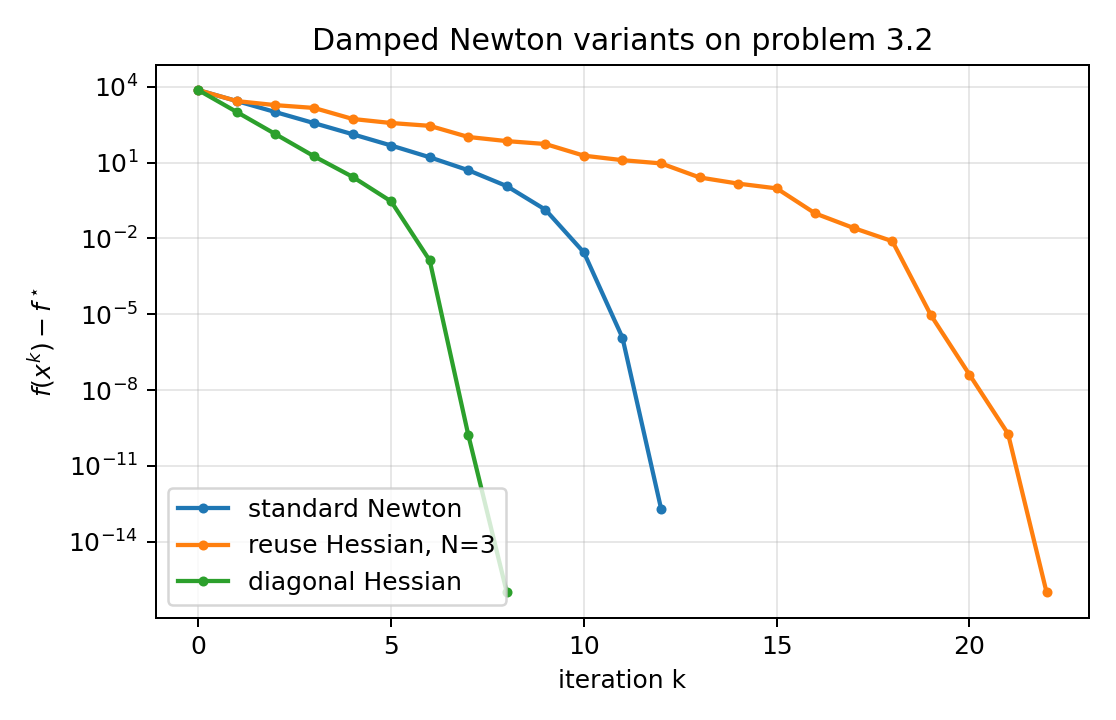
\includegraphics[width=0.72\textwidth]{hw12_3_2_newton_variants.png}
  \end{center}

  \item[(c)]
  对重复利用 Hessian 的方法，本实验取 $N=3$，也就是每 $3$ 次迭代重新计算一次 Hessian，其余迭代复用上一次记录的 Hessian。对角估计方法取
  \[
    D_k=\operatorname{diag}(\nabla^2 f(x_k)),
    \qquad
    d_k=-D_k^{-1}\nabla f(x_k).
  \]
  三种方法都使用相同的回溯线搜索和停止准则。结果如下。

  \begin{center}
  \renewcommand{\arraystretch}{1.25}
  \begin{tabular}{|c|c|c|c|}
  \hline
  方法 & 迭代次数 & Hessian 计算次数 & 最终误差 $f(x_k)-f^\star$\\
  \hline
  常规阻尼 Newton & 12 & 12 & $2.074\times10^{-13}$\\
  \hline
  重复利用 Hessian, $N=3$ & 22 & 8 & $0$（数值精度下）\\
  \hline
  对角 Hessian 估计 & 8 & 8 & $0$（数值精度下）\\
  \hline
  \end{tabular}
  \end{center}

  可以看到，重复利用 Hessian 减少了 Hessian 计算次数，但迭代次数增加；对角估计每步方向更便宜，且在这个二维例子中表现很好。不过这并不说明对角估计总是优于 Newton 法，因为它忽略了不同坐标之间的曲率耦合，在高维强耦合问题中可能需要更多迭代。
\end{enumerate}




\section{拟牛顿法}

\paragraph{4.1}
线搜索是优化方法中的一个重要步骤。我们已经了解了基本的回溯线搜索(\textbf{Armijo-Wolfe 线搜索})是一种重要的非精确线搜索。假设我们希望找到 $t$，使得
$f(x_k+t_kd_k) \approx \min_{t} f(x_k+td_k)$，
其中 $d_k$ 是第 $k$ 步的搜索方向；在梯度法中，$d_k=-\nabla f(x)$，而在牛顿法中，$d_k=-\nabla^2 f(x)^{-1} \nabla f(x)$。

更进一步，为了描述这些线搜索条件，取参数 $0<c_1<c_2<1$，得到两个条件


$$\textbf{充分下降条件：} f(x_k+t_k d_k) \leq f(x_k) +c_1t_k\nabla f(x_k)^T d_k$$

$$\textbf{曲率条件：} \nabla f(x_k+t_kd_k)^Td_k \geq c_2 \nabla f(x_k)^Td_k$$

(如果定义 $g(t)=f(x_k+td_k)$，那么曲率条件就是 $g'(t_k)\geq c_2 g'(0)$）

这两个条件合在一起称为（弱）Wolfe 条件。可以证明，只要 $d$ 是一个下降方向，集合 $\{t\;|\; t \text{ 满足 Wolfe 条件}\}$ 就有非空的内部。[《数值优化》（Nocedal 和 Wright），第 3 章]

该线搜索可以利用如下二分法求解：


\begin{algorithm}[H]
	\SetAlgoLined
	
	Initialization: Choose $0<c_1<c_2<1$, and set $t=1$, $\alpha=0$, $\beta=+\infty$\;
	\While{True}{
		
		\uIf{$f(x+td)>f(x)+c_1t\nabla f(x)^T d$}{
			set $\beta=t$ and reset $t=\frac{1}{2}(\alpha+\beta)$ \;
		}
		\uElseIf{$\nabla f(x+td)^Td < c_2 \nabla f(x)^Td$}{
			set $\alpha=t$, and reset $t = \begin{cases}2 \alpha, & \mbox{if } \beta=+\infty \\ \frac{1}{2}(\alpha+\beta), & \mbox{Otherwise }\end{cases}$\
		}
		\Else{
			break \;
		}
		
	}
\end{algorithm}

\begin{enumerate}
	\item[(a)] 编程实现采用Wolfe线搜索的BFGS方法，利用其求解3.2 (b)的问题，并与牛顿法进行比较。
	
	\item[(b)] 考虑非平滑凸问题$f(u,v)=|u|+3v^2$，利用梯度下降法与BFGS方法，采用Wolfe线搜索进行求解。如果随机生成$u_0 \neq 0$ 和 $v_0 \neq 0$的初始点, 两个方法收敛吗？ (注意：迭代过程将永远无法触及$u_i=0$区域，所以各个点都局部可微的 )
	
	画出$f(x_k)- f^*$ 与迭代次数 $k$直接的关系，并解释结果。
	
	\item[(c)] 考虑如下问题$f(u,v)=|u|^3+v+\frac{1}{2}v^2$，编程实现梯度下降法、近端梯度法、牛顿法、拟牛顿法求解，要求与上题一致。
	
\end{enumerate}

\textbf{解：}
\begin{enumerate}
  \item[(a)]
  BFGS 方法维护逆 Hessian 的近似矩阵 $B_k$，搜索方向为
  \[
    d_k=-B_k\nabla f(x_k).
  \]
  采用题中 Wolfe 线搜索得到步长 $t_k$ 后，更新
  \[
    x_{k+1}=x_k+t_kd_k.
  \]
  记
  \[
    s_k=x_{k+1}-x_k,\qquad
    y_k=\nabla f(x_{k+1})-\nabla f(x_k),
  \]
  若 $y_k^Ts_k>0$，则逆 Hessian 近似按
  \[
    B_{k+1}
    =
    (I-\rho_ks_ky_k^T)B_k(I-\rho_ky_ks_k^T)
    +\rho_ks_ks_k^T,
    \qquad
    \rho_k=\frac1{y_k^Ts_k}
  \]
  更新。初始取 $B_0=I$。

  对 3.2(b) 的问题，从同一初始点 $x_0=(5,2)^T$ 出发，BFGS 采用 Wolfe 线搜索，停止准则仍取 $f(x_k)-f^\star<10^{-10}$。数值结果为
  \[
    k=23,\qquad
    x_k\approx(-0.33650818,\ 0.08109314)^T,
    \qquad
    f(x_k)-f^\star\approx7.040\times10^{-12}.
  \]
  与阻尼 Newton 法相比，BFGS 不需要显式计算 Hessian，但迭代次数更多。

  \begin{center}
    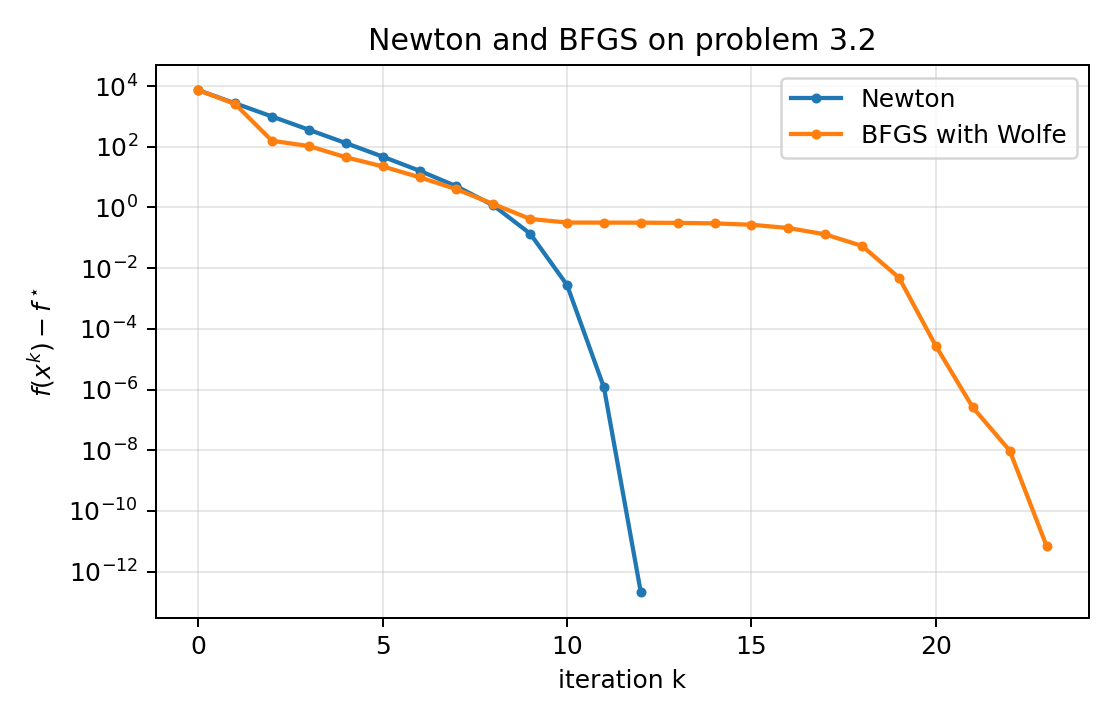
\includegraphics[width=0.72\textwidth]{hw12_4_1a_bfgs_vs_newton.png}
  \end{center}

  \item[(b)]
  该问题的最优解为
  \[
    (u^\star,v^\star)=(0,0),
    \qquad
    f^\star=0.
  \]
  在 $u\ne0$ 的区域，局部梯度为
  \[
    \nabla f(u,v)=
    \begin{bmatrix}
      \operatorname{sign}(u)\\
      6v
    \end{bmatrix}.
  \]
  本实验随机生成初始点
  \[
    x_0=(u_0,v_0)^T\approx(2.21330492,\ -1.81250263)^T.
  \]
  用 Wolfe 线搜索分别实现梯度下降法和 BFGS 方法，得到如下结果。

  \begin{center}
    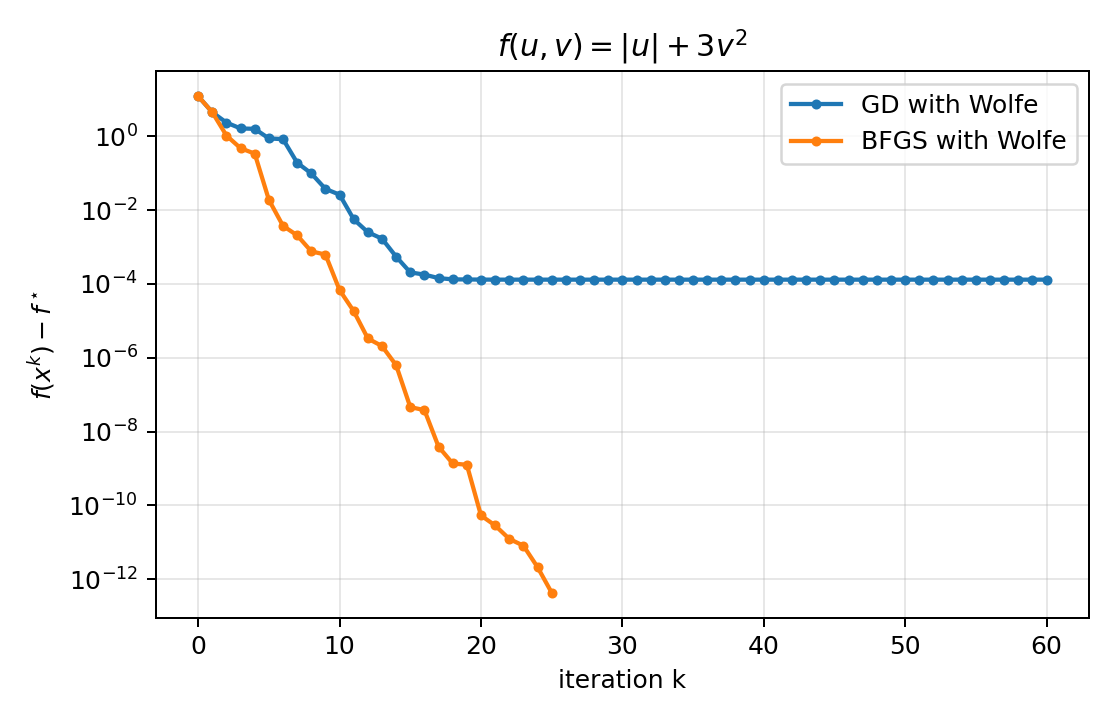
\includegraphics[width=0.72\textwidth]{hw12_4_1b_abs_quad.png}
  \end{center}

  数值上，两种方法的函数值都收敛到 $f^\star=0$。梯度下降法在 $60$ 次迭代后达到
  \[
    f(x_k)-f^\star\approx1.302\times10^{-4},
  \]
  BFGS 在 $25$ 次迭代后达到
  \[
    f(x_k)-f^\star\approx4.341\times10^{-13}.
  \]
  但是需要注意，$|u|$ 在 $u=0$ 处不可微，所以普通光滑优化中的 Wolfe-BFGS 收敛理论不能直接套用。这里的收敛是该具体数值实验中的现象；对一般非光滑问题，BFGS 可能出现不稳定或无法保证收敛。

  \item[(c)]
  对
  \[
    f(u,v)=|u|^3+v+\frac12v^2
  \]
  有
  \[
    f(u,v)=|u|^3+\frac12(v+1)^2-\frac12,
  \]
  因此
  \[
    (u^\star,v^\star)=(0,-1),
    \qquad
    f^\star=-\frac12.
  \]
  该函数虽然含有绝对值，但 $|u|^3$ 在 $u=0$ 处仍然可微，梯度为
  \[
    \nabla f(u,v)
    =
    \begin{bmatrix}
      3u|u|\\
      1+v
    \end{bmatrix}.
  \]
  Newton 法使用 Hessian
  \[
    \nabla^2 f(u,v)
    =
    \begin{bmatrix}
      6|u| & 0\\
      0 & 1
    \end{bmatrix},
  \]
  当 $u$ 很接近 $0$ 时，$u$ 方向曲率接近退化，因此实际实现中需要谨慎处理。

  近端梯度法把 $|u|^3$ 作为近端项，把
  \[
    q(v)=v+\frac12v^2
  \]
  作为光滑项。对标量问题
  \[
    \operatorname{prox}_{t|\cdot|^3}(z)
    =
    \arg\min_s
    \left\{
      \frac1{2t}(s-z)^2+|s|^3
    \right\},
  \]
  最优解与 $z$ 同号。令 $r=|s|$，一阶条件给出
  \[
    r+3tr^2=|z|.
  \]
  所以
  \[
    \operatorname{prox}_{t|\cdot|^3}(z)
    =
    \operatorname{sign}(z)
    \frac{-1+\sqrt{1+12t|z|}}{6t}.
  \]

  从与上一小题相同的初始点出发，比较梯度下降、近端梯度、Newton 和 BFGS，结果如下。

  \begin{center}
    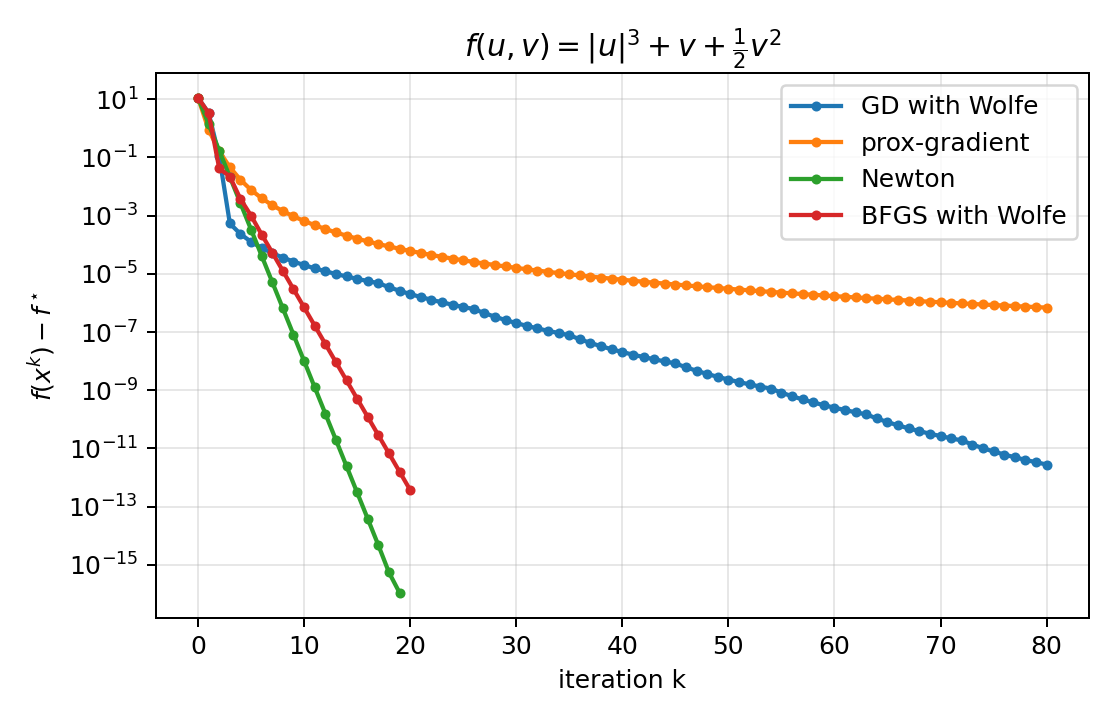
\includegraphics[width=0.72\textwidth]{hw12_4_1c_abs3.png}
  \end{center}

  在本实验中，Newton 法 $19$ 次迭代后达到数值精度，BFGS 用 $20$ 次迭代达到 $3.760\times10^{-13}$ 的误差；梯度下降在 $80$ 次迭代后误差约为 $2.817\times10^{-12}$；近端梯度法稳定但较慢，$80$ 次迭代后误差约为 $6.892\times10^{-7}$。
\end{enumerate}

\paragraph{4.2}
比较一阶算法、二阶算法、与拟牛顿法的优劣。

\textbf{解：}
一阶算法、二阶算法和拟 Newton 法的核心区别在于使用的信息量不同：一阶算法只使用梯度或次梯度，二阶算法直接使用 Hessian，拟 Newton 法不直接计算 Hessian，而是用历史迭代中的 $s_k$ 和 $y_k$ 学习曲率。

\begin{center}
\renewcommand{\arraystretch}{1.35}
\begin{tabular}{|p{2.7cm}|p{4.0cm}|p{4.0cm}|p{4.0cm}|}
\hline
类别 & 优点 & 缺点 & 适用场景\\
\hline
一阶算法
& 单步计算便宜；实现简单；适合大规模问题；能自然扩展到随机优化、投影和近端框架
& 只利用坡度信息，对条件数敏感；在病态问题中容易 zig-zag；高精度收敛通常较慢
& 大规模机器学习、有限和问题、简单约束或复合结构问题 \\
\hline
二阶算法
& 利用 Hessian 曲率信息；方向质量高；对病态问题更有效；在最优点附近常有二次收敛
& Hessian 计算和存储成本高；每步通常要求解线性方程组；非凸时 Hessian 可能不正定
& 中小规模、高精度、光滑优化问题 \\
\hline
拟 Newton 法
& 不直接计算 Hessian；通过梯度差学习曲率；通常比一阶法快；BFGS 局部可超线性收敛
& 完整 BFGS 仍需 $O(n^2)$ 存储；非光滑问题中理论保证弱；曲率近似质量依赖线搜索和更新条件
& 中等规模光滑优化；大规模问题可用 L-BFGS \\
\hline
\end{tabular}
\end{center}

总体来看，一阶算法适合“大规模、低单步成本、允许中等精度”的场景；二阶算法适合“中小规模、高精度、光滑且 Hessian 可承受”的场景；拟 Newton 法处在两者之间，是实践中常用的折中方案。若维度非常高，通常优先考虑 SGD、Adam 或 L-BFGS；若维度不高且需要高精度，则 Newton 或阻尼 Newton 往往更合适。

\appendix
\section{第 3、4 部分代码}
第 3.2 与第 4.1 的图像由以下 Python 代码生成。

\lstinputlisting[language=Python]{generate_figures.py}




\end{document}
